% Copyright 2018 Melvin Eloy Irizarry-Gelpí
\setcounter{chapter}{7}
\chapter{Kinetic and Gravitational Energy}
%%%%%%%%%%%%%%%%%%%%%%%%%%%%%%%%%%%%%%%%%%%%%%%%%%%%%%%%%%%%%%%%%%%%%%%%%%%%%%%%
In this experiment you will study the dependance of gravitational energy on height.
%%%%%%%%%%%%%%%%%%%%%%%%%%%%%%%%%%%%%%%%%%%%%%%%%%%%%%%%%%%%%%%%%%%%%%%%%%%%%%%%
\section{Preliminary}
%%%%%%%%%%%%%%%%%%%%%%%%%%%%%%%%%%%%%%%%%%%%%%%%%%%%%%%%%%%%%%%%%%%%%%%%%%%%%%%%
In the previous experiment, you encountered \textbf{kinetic} energy (the energy associated to being in motion), \textbf{elastic} energy (the potential energy associated to deforming a spring), and \textbf{mechanic} energy (the sum of kinetic and potential energy).

The amount of \textbf{kinetic} energy $K$ depends on the amount of mass $m$ and speed $v$:
\begin{equation}
    K = \frac{1}{2} m v^{2}
\end{equation}
Note that kinetic energy changes if the speed of the object changes.

Another form of energy is \textbf{gravitational} energy (a form of \textbf{potential} energy), which is associated to being in a region with a gravitational field. The amount of gravitational energy $U_{g}$ depends on the amount of mass $m$, the amount of gravitational acceleration $g$, and the amount of height $h$ measured from a fixed reference point:
\begin{equation}
    U_{g} = m g h
\end{equation}
Note that the gravitational energy changes if the height of the object changes. Recall that, on the surface of Earth, $g = 9.80$ m/s$^{2}$.

Finally, you have \textbf{mechanic} energy. The amount of mechanic energy $E$ is the sum of kinetic energy $K$ and potential energy. For the previous experiment, the potential energy was only elastic energy because you had a spring and the object moved along a horizontal track. In the case when the potential energy is only gravitational in nature, the mechanic energy is
\begin{equation}
    E = K + U_{g}
\end{equation}
Energy cannot be created nor destroyed; it can only be transformed into other forms of energy. In a closed system, where energy is not added nor removed by an external source, mechanic energy $E$ is \textbf{constant in time}.

If the object only moves and feels gravity, then the mechanic energy $E$ is given by
\begin{equation}
    E = \frac{1}{2} m v^{2} + m g h
\end{equation}
Solving for $v^{2}$ you get
\begin{equation}
    v^{2} = \left( - 2 g \right) h + \left( \frac{2 E}{m} \right)
    \label{eq.07.vv}
\end{equation}
This relation predicts that $v^{2}$ is a \textbf{linear function} of $h$ with the \textbf{slope} being $-2g$ and the \textbf{intercept} being $2 E / m$. That is, the data in a $v^{2}$ versus $h$ chart should have a \textbf{linear shape}.
%%%%%%%%%%%%%%%%%%%%%%%%%%%%%%%%%%%%%%%%%%%%%%%%%%%%%%%%%%%%%%%%%%%%%%%%%%%%%%%%
\section{Experiment}
%%%%%%%%%%%%%%%%%%%%%%%%%%%%%%%%%%%%%%%%%%%%%%%%%%%%%%%%%%%%%%%%%%%%%%%%%%%%%%%%
In order to study a system where there is gravitational energy, and also that the gravitational energy changes with time, you used an object moving along an inclined track. With a motion sensor, you recorded the \textbf{position} $d$ and \textbf{velocity} $v$ along the incline as they changed with time. You also recorded some height measurements to determine the sine of the angle of inclination of the inclined track. Also, you recorded the mass $m$ of the cart.
%%%%%%%%%%%%%%%%%%%%%%%%%%%%%%%%%%%%%%%%%%%%%%%%%%%%%%%%%%%%%%%%%%%%%%%%%%%%%%%%
\section{Analysis}
%%%%%%%%%%%%%%%%%%%%%%%%%%%%%%%%%%%%%%%%%%%%%%%%%%%%%%%%%%%%%%%%%%%%%%%%%%%%%%%%
You would like to test two predictions:
\begin{enumerate}
    \item Mechanic energy does not change with time.
    \item There is a linear relation between $v^{2}$ and $h$ given by Equation \ref{eq.07.vv}.
\end{enumerate}
To test the first prediction, you need to compute the mechanic energy with the data that you collected. To test the second prediction, you need to make a graph with $v^{2}$ in the vertical axis and $h$ in the horizontal axis. Here are some steps to complete the analysis.
%%%%%%%%%%%%%%%%%%%%%%%%%%%%%%%%%%%%%%%%%%%%%%%%%%%%%%%%%%%%%%%%%%%%%%%%%%%%%%%%
\subsection{Truncate the Data}
%%%%%%%%%%%%%%%%%%%%%%%%%%%%%%%%%%%%%%%%%%%%%%%%%%%%%%%%%%%%%%%%%%%%%%%%%%%%%%%%
Before you can do anything with the data from the experiment, you need to isolated the part of the data where the motion along the incline is happening. In order to know where to cut the data, it is best to make a scatter chart with \textbf{velocity} in the vertical axis and \textbf{time} in the horizontal axis. There are three kinds of truncation:
\begin{enumerate}
    \item Upward motion only: find the time just after the velocity values begin the diagonal downward trend, and the time when the velocity is close to zero
    \item Downward motion only: find the time when the velocity is close to zero, and the time just before the velocity ends the diagonal downward trend
    \item Upward and downward motion: find the time just after the velocity values begin the diagonal downward trend, and the time just before the downward trend ends
\end{enumerate}
Once you know the initial time and the final time of the motion, just delete the data outside of this time interval.

However, for convenience, you might want to truncate the data as a last step, after calculating everything for one full run, and duplicating the sheet for the other runs.
%%%%%%%%%%%%%%%%%%%%%%%%%%%%%%%%%%%%%%%%%%%%%%%%%%%%%%%%%%%%%%%%%%%%%%%%%%%%%%%%
\subsection{Kinetic Energy}
%%%%%%%%%%%%%%%%%%%%%%%%%%%%%%%%%%%%%%%%%%%%%%%%%%%%%%%%%%%%%%%%%%%%%%%%%%%%%%%%
Here are the steps to follow to calculate the kinetic energy at each moment in time.
%%%%%%%%%%%%%%%%%%%%%%%%%%%%%%%%%%%%%%%%%%%%%%%%%%%%%%%%%%%%%%%%%%%%%%%%%%%%%%%%
\subsubsection{Calculate the Squared Velocity}
%%%%%%%%%%%%%%%%%%%%%%%%%%%%%%%%%%%%%%%%%%%%%%%%%%%%%%%%%%%%%%%%%%%%%%%%%%%%%%%%
In a separate column, you should calculate the squared velocity using the values in the velocity column.
%%%%%%%%%%%%%%%%%%%%%%%%%%%%%%%%%%%%%%%%%%%%%%%%%%%%%%%%%%%%%%%%%%%%%%%%%%%%%%%%
\subsubsection{Calculate the Kinetic Energy}
%%%%%%%%%%%%%%%%%%%%%%%%%%%%%%%%%%%%%%%%%%%%%%%%%%%%%%%%%%%%%%%%%%%%%%%%%%%%%%%%
In a separate column, you should compute the value of the kinetic energy using the values in the squared velocity column. If $v$ is a velocity value, then the corresponding kinetic energy is given by
\begin{equation}
    K = \frac{1}{2} m v^{2}
\end{equation}
For the mass, you should use the value of the mass of the cart that you measured with the electronic scale. See Table \ref{table:07.mass} for my case.
%%%%%%%%%%%%%%%%%%%%%%%%%%%%%%%%%%%%%%%%%%%%%%%%%%%%%%%%%%%%%%%%%%%%%%%%%%%%%%%%
\subsection{Gravitational Energy}
%%%%%%%%%%%%%%%%%%%%%%%%%%%%%%%%%%%%%%%%%%%%%%%%%%%%%%%%%%%%%%%%%%%%%%%%%%%%%%%%
Here are the steps to follow to calculate the gravitational energy at each moment in time.
%%%%%%%%%%%%%%%%%%%%%%%%%%%%%%%%%%%%%%%%%%%%%%%%%%%%%%%%%%%%%%%%%%%%%%%%%%%%%%%%
\subsubsection{Calculate the Sine of the Angle of Inclination}
%%%%%%%%%%%%%%%%%%%%%%%%%%%%%%%%%%%%%%%%%%%%%%%%%%%%%%%%%%%%%%%%%%%%%%%%%%%%%%%%
You measured the heights of four positions along the incline. Table \ref{table:07.x} has the position values along the track and Tables \ref{table:07.h.1} and Table \ref{table:07.h.2} have the height values. The value of the sine can be found by calculating a ratio of differences. Table \ref{table:07.sine.1} and Table \ref{table:07.sine.2} have three sine calculations for both one-box and two-box inclined tracks.
%%%%%%%%%%%%%%%%%%%%%%%%%%%%%%%%%%%%%%%%%%%%%%%%%%%%%%%%%%%%%%%%%%%%%%%%%%%%%%%%
\subsubsection{Calculate Height}
%%%%%%%%%%%%%%%%%%%%%%%%%%%%%%%%%%%%%%%%%%%%%%%%%%%%%%%%%%%%%%%%%%%%%%%%%%%%%%%%
In a separate column, you should compute the value of the height at the incline using the values in the position column and the sine. If $d$ is a position value, then the corresponding height is given by
\begin{equation}
    h = d \sin(\theta)
\end{equation}
For sine, use the average of the three sine values you found.
%%%%%%%%%%%%%%%%%%%%%%%%%%%%%%%%%%%%%%%%%%%%%%%%%%%%%%%%%%%%%%%%%%%%%%%%%%%%%%%%
\subsubsection{Calculate Gravitational Energy}
%%%%%%%%%%%%%%%%%%%%%%%%%%%%%%%%%%%%%%%%%%%%%%%%%%%%%%%%%%%%%%%%%%%%%%%%%%%%%%%%
In a separate column, you should compute the value of the gravitational energy using the values in the height column. If $h$ is a height value, then the corresponding gravitational energy is given by
\begin{equation}
    U_{g} = m g h
\end{equation}
For $g$, use the accepted value of 9.80 m/s$^{2}$.
%%%%%%%%%%%%%%%%%%%%%%%%%%%%%%%%%%%%%%%%%%%%%%%%%%%%%%%%%%%%%%%%%%%%%%%%%%%%%%%%
\subsection{Mechanic Energy}
%%%%%%%%%%%%%%%%%%%%%%%%%%%%%%%%%%%%%%%%%%%%%%%%%%%%%%%%%%%%%%%%%%%%%%%%%%%%%%%%
Here are the steps to follow to find the mechanic energy.
%%%%%%%%%%%%%%%%%%%%%%%%%%%%%%%%%%%%%%%%%%%%%%%%%%%%%%%%%%%%%%%%%%%%%%%%%%%%%%%%
\subsubsection{Calculate the Mechanic Energy}
%%%%%%%%%%%%%%%%%%%%%%%%%%%%%%%%%%%%%%%%%%%%%%%%%%%%%%%%%%%%%%%%%%%%%%%%%%%%%%%%
In a separate column, you should compute the value of the mechanic energy using the values in the kinetic and gravitational energy columns. If $K$ is a value in the kinetic energy column, and $U_{g}$ is a value in the gravitational energy column, then the mechanic energy is given by
\begin{equation}
    E = K + U_{g}
\end{equation}
Make sure that you add values that are evaluated at the same time.
%%%%%%%%%%%%%%%%%%%%%%%%%%%%%%%%%%%%%%%%%%%%%%%%%%%%%%%%%%%%%%%%%%%%%%%%%%%%%%%%
\subsubsection{Calculate the Time-Average Mechanic Energy}
%%%%%%%%%%%%%%%%%%%%%%%%%%%%%%%%%%%%%%%%%%%%%%%%%%%%%%%%%%%%%%%%%%%%%%%%%%%%%%%%
Once you have a column with the mechanic energy values over time, you can calculate the average value of that column and find the \textbf{time-average value of mechanic energy}.
%%%%%%%%%%%%%%%%%%%%%%%%%%%%%%%%%%%%%%%%%%%%%%%%%%%%%%%%%%%%%%%%%%%%%%%%%%%%%%%%
\subsection{Visualize Mechanic Energy versus Time}
%%%%%%%%%%%%%%%%%%%%%%%%%%%%%%%%%%%%%%%%%%%%%%%%%%%%%%%%%%%%%%%%%%%%%%%%%%%%%%%%
One of the goals of this experiment is to verify that \textbf{mechanic energy is constant in time}. To check this, you can make a scatter chart with time in the horizontal axis and mechanic energy in the vertical axis.

In principle, you should see that the values of mechanic energy do not change with time. In practice, we see that in general the mechanic energy decreases as time passes. This is actually true, since in this experiment you could not completely remove friction and this force leads to \textbf{a loss of energy} to the environment. However, the amount of change in energy over time is very small, so effectively (and approximately) mechanic energy is almost constant.
%%%%%%%%%%%%%%%%%%%%%%%%%%%%%%%%%%%%%%%%%%%%%%%%%%%%%%%%%%%%%%%%%%%%%%%%%%%%%%%%
\subsection{Visualize Squared Velocity versus Height}
%%%%%%%%%%%%%%%%%%%%%%%%%%%%%%%%%%%%%%%%%%%%%%%%%%%%%%%%%%%%%%%%%%%%%%%%%%%%%%%%
The other goal of this experiment was to verify the linear relation suggested by Equation \ref{eq.07.vv} between $v^{2}$ and $h$ due to conservation of energy. Since the relation is a linear function, the data points should arrange themselves to form a linear shape.

If the data were perfect, then the \textbf{slope} of this linear fit should be given by
\begin{equation} \label{eq.07.slope}
    \text{slope} = -2g = -19.6 \text{ m/s}^{2}
\end{equation}
and the \textbf{intercept} would be related to the amount of mechanic energy via
\begin{equation}
    \text{intercept} = \frac{2 E}{m}
\end{equation}
The slope is negative, so you should see a diagonal line that is downward as height increases. From the intercept you can get a value for mechanic energy that should be close to what you found in the mechanic energy column:
\begin{equation} \label{eq.07.intercept}
    E = \frac{m \times \text{ intercept}}{2}
\end{equation}
You can also compare this value with the time-average value of the mechanic energy.
%%%%%%%%%%%%%%%%%%%%%%%%%%%%%%%%%%%%%%%%%%%%%%%%%%%%%%%%%%%%%%%%%%%%%%%%%%%%%%%%
\section{My Data}
%%%%%%%%%%%%%%%%%%%%%%%%%%%%%%%%%%%%%%%%%%%%%%%%%%%%%%%%%%%%%%%%%%%%%%%%%%%%%%%%
I collected six runs of data:
\begin{itemize}
    \item Runs 1, 2, and 3: one box of height
    \item Runs 4, 5, and 6: two boxes of height
\end{itemize}
Here are the truncations I used on the spreadsheet:
\begin{itemize}
    \item Run 1 and 4: Upward motion only
    \item Run 2 and 5: Downward motion only
    \item Run 3 and 6: Upward and downward motion
\end{itemize}
As you can see from Figure \ref{figure:07.v2.1} Figure \ref{figure:07.v2.2} and Figure \ref{figure:07.v2.3} the relation between $v^{2}$ and $h$ was found to be very linear. From the best fit line you can find the slope and the intercept. From the intercept, you can use Equation \ref{eq.07.intercept} to find an estimate of the mechanic energy. You can compare this estimate to the time-average value of mechanic energy. Table \ref{table.07.results} summarizes my results.

Although the mechanic energy was found to not be constant in time, as you can see from Figure \ref{figure.07.run.4.e}, Figure \ref{figure.07.run.5.e}, and Figure \ref{figure.07.run.6.e}, the change in energy is very small. Another important feature is that the mechanic energy is almost always getting slightly smaller. This can be explained as due to friction doing a negative amount of work that leads to a loss of mechanic energy.
%%%%%%%%%%%%%%%%%%%%%%%%%%%%%%%%%%%%%%%%%%%%%%%%%%%%%%%%%%%%%%%%%%%%%%%%%%%%%%%%
\section{Your Data}
%%%%%%%%%%%%%%%%%%%%%%%%%%%%%%%%%%%%%%%%%%%%%%%%%%%%%%%%%%%%%%%%%%%%%%%%%%%%%%%%
You should have six runs of data:
\begin{itemize}
    \item Three runs with one box of height.
    \item Three runs with two boxes of height.
\end{itemize}
Each run should consist of the cart moving upward first, and then downward before being stopped.
%%%%%%%%%%%%%%%%%%%%%%%%%%%%%%%%%%%%%%%%%%%%%%%%%%%%%%%%%%%%%%%%%%%%%%%%%%%%%%%%
\newpage
\section{Your Laboratory Report}
%%%%%%%%%%%%%%%%%%%%%%%%%%%%%%%%%%%%%%%%%%%%%%%%%%%%%%%%%%%%%%%%%%%%%%%%%%%%%%%%
Your lab report should include the following:
\begin{itemize}
    \item Tables where you show the three estimates of the sine function for both heights, as well as the average (see Table \ref{table:07.sine.1} and Table \ref{table:07.sine.2})
    \item A table with your results for the slope, the time-average value of $E$, and the estimate of $E$ from the intercept, similar to Table \ref{table.07.results}.
    \item One scatter chart with $v^{2}$ in the vertical axis and $h$ in the horizontal axis for \textbf{upward motion} only (see Figure \ref{figure:07.v2.1}). Include the best-fit line.
    \item One scatter chart with $v^{2}$ in the vertical axis and $h$ in the horizontal axis for \textbf{downward motion} only (see Figure \ref{figure:07.v2.2}). Include the best-fit line.
    \item One scatter chart with $v^{2}$ in the vertical axis and $h$ in the horizontal axis for \textbf{both upward and downward motion} (see Figure \ref{figure:07.v2.3}). Include the best-fit line.
    \item One scatter chart with mechanic energy in the vertical axis and time in the horizontal axis for \textbf{upward motion} only (see Figure \ref{figure.07.run.4.e}).
    \item One scatter chart with mechanic energy in the vertical axis and time in the horizontal axis for \textbf{downward motion} only (see Figure \ref{figure.07.run.5.e}).
    \item One scatter chart with mechanic energy in the vertical axis and time in the horizontal axis for \textbf{both upward and downward motion} (see Figure \ref{figure.07.run.6.e}).
\end{itemize}
You should also answer the following questions:
\begin{enumerate}
    \item Are your results for the slope consistent for the three motions considered (upward only, downward only, both upward and downward)?
    \item Did you find mechanic energy to be approximately constant? Or did it changed by a large amount?
    \item If mechanic energy was not found to be constant, did it mostly decrease?
\end{enumerate}
%%%%%%%%%%%%%%%%%%%%%%%%%%%%%%%%%%%%%%%%%%%%%%%%%%%%%%%%%%%%%%%%%%%%%%%%%%%%%%%%
\FloatBarrier
\newpage
\section{Tables}
%%%%%%%%%%%%%%%%%%%%%%%%%%%%%%%%%%%%%%%%%%%%%%%%%%%%%%%%%%%%%%%%%%%%%%%%%%%%%%%%
\begin{table}[ht]
    \centering
    \begin{tabular}{|l|r|}
        \hline
        Name & Value (cm) \\
        \hline
        $x_{1}$ & 25 \\
        $x_{2}$ & 50 \\
        $x_{3}$ & 75 \\
        $x_{4}$ & 100 \\
        \hline
    \end{tabular}
    \caption{Position values for both one-box and two-box heights}
    \label{table:07.x}
\end{table}
%%%%%%%%%%%%%%%%%%%%%%%%%%%%%%%%%%%%%%%%%%%%%%%%%%%%%%%%%%%%%%%%%%%%%%%%%%%%%%%%
\begin{table}[ht]
    \centering
    \begin{tabular}{|l|r|}
        \hline
        Name & Value (cm) \\
        \hline
        $h_{1}$ & 4.3 \\
        $h_{2}$ & 6.1 \\
        $h_{3}$ & 8 \\
        $h_{4}$ & 10 \\
        \hline
    \end{tabular}
    \caption{Height values for one-box height}
    \label{table:07.h.1}
\end{table}
%%%%%%%%%%%%%%%%%%%%%%%%%%%%%%%%%%%%%%%%%%%%%%%%%%%%%%%%%%%%%%%%%%%%%%%%%%%%%%%%
\begin{table}[ht]
    \centering
    \begin{tabular}{|l|r|}
        \hline
        Name & Value (cm) \\
        \hline
        $h_{1}$ & 5.2 \\
        $h_{2}$ & 8.4 \\
        $h_{3}$ & 11.7 \\
        $h_{4}$ & 15 \\
        \hline
    \end{tabular}
    \caption{Height values for two-box height}
    \label{table:07.h.2}
\end{table}
%%%%%%%%%%%%%%%%%%%%%%%%%%%%%%%%%%%%%%%%%%%%%%%%%%%%%%%%%%%%%%%%%%%%%%%%%%%%%%%%
\begin{table}[ht]
    \centering
    \begin{tabular}{|l|r|}
        \hline
        Name & Value (no units) \\
        \hline
        $\left( h_{2} - h_{1} \right) / \left( x_{2} - x_{1} \right)$ & 0.072 \\
        $\left( h_{3} - h_{2} \right) / \left( x_{3} - x_{2} \right)$ & 0.076 \\
        $\left( h_{4} - h_{3} \right) / \left( x_{4} - x_{3} \right)$ & 0.080 \\
        \hline
        Average Sine & 0.076 \\
        \hline
    \end{tabular}
    \caption{Sine values for one-box height}
    \label{table:07.sine.1}
\end{table}
%%%%%%%%%%%%%%%%%%%%%%%%%%%%%%%%%%%%%%%%%%%%%%%%%%%%%%%%%%%%%%%%%%%%%%%%%%%%%%%%
\begin{table}[ht]
    \centering
    \begin{tabular}{|l|r|}
        \hline
        Name & Value (no units) \\
        \hline
        $\left( h_{2} - h_{1} \right) / \left( x_{2} - x_{1} \right)$ & 0.128 \\
        $\left( h_{3} - h_{2} \right) / \left( x_{3} - x_{2} \right)$ & 0.132 \\
        $\left( h_{4} - h_{3} \right) / \left( x_{4} - x_{3} \right)$ & 0.132 \\
        \hline
        Average Sine & 0.131 \\
        \hline
    \end{tabular}
    \caption{Sine values for two-box height}
    \label{table:07.sine.2}
\end{table}
%%%%%%%%%%%%%%%%%%%%%%%%%%%%%%%%%%%%%%%%%%%%%%%%%%%%%%%%%%%%%%%%%%%%%%%%%%%%%%%%
\begin{table}[ht]
    \centering
    \begin{tabular}{|l|r|}
        \hline
        Name & Value (kg) \\
        \hline
        Mass of cart & 0.5087 \\
        \hline
    \end{tabular}
    \caption{Mass measurements}
    \label{table:07.mass}
\end{table}
%%%%%%%%%%%%%%%%%%%%%%%%%%%%%%%%%%%%%%%%%%%%%%%%%%%%%%%%%%%%%%%%%%%%%%%%%%%%%%%%
\begin{table}[ht]
    \centering
    \begin{tabular}{|l|r|r|r|}
        \hline
        Run & Slope (m/s$^{2}$) & $E$ from Intercept (J) & Time-Average $E$ (J) \\
        \hline
        1 & -21.47 & 0.3157 & 0.2939 \\
        2 & -16.84 & 0.2459 & 0.2788 \\
        3 & -18.98 & 0.3065 & 0.3143 \\
        4 & -20.75 & 0.5010 & 0.4779 \\
        5 & -17.62 & 0.4318 & 0.4689 \\
        6 & -18.97 & 0.4979 & 0.5109 \\
        \hline
    \end{tabular}
    \caption{Summary of results}
    \label{table.07.results}
\end{table}
%%%%%%%%%%%%%%%%%%%%%%%%%%%%%%%%%%%%%%%%%%%%%%%%%%%%%%%%%%%%%%%%%%%%%%%%%%%%%%%%
\FloatBarrier
\newpage
\section{Figures}
%%%%%%%%%%%%%%%%%%%%%%%%%%%%%%%%%%%%%%%%%%%%%%%%%%%%%%%%%%%%%%%%%%%%%%%%%%%%%%%%
\begin{figure}[ht]
    \centering
    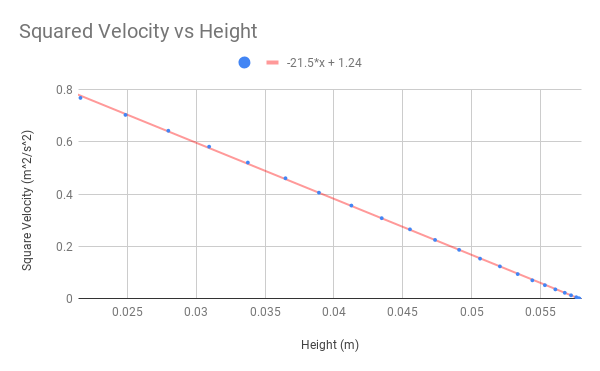
\includegraphics[scale=0.71]{image/07-mechanic/v2-uphill.png}
    \caption{$v^{2}$ versus $h$ for Run 1: Upward motion only}
    \label{figure:07.v2.1}
\end{figure}
%%%%%%%%%%%%%%%%%%%%%%%%%%%%%%%%%%%%%%%%%%%%%%%%%%%%%%%%%%%%%%%%%%%%%%%%%%%%%%%%
\begin{figure}[ht]
    \centering
    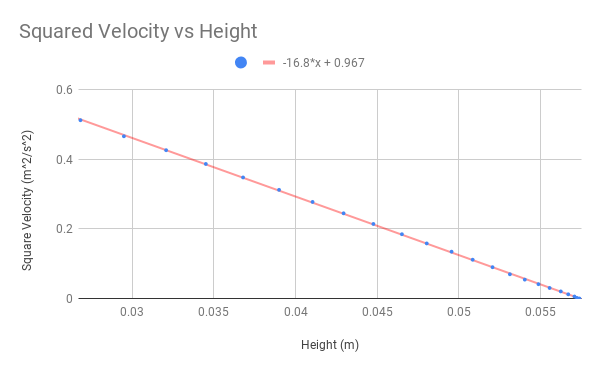
\includegraphics[scale=0.71]{image/07-mechanic/v2-downhill.png}
    \caption{$v^{2}$ versus $h$ for Run 2: Downward motion only}
    \label{figure:07.v2.2}
\end{figure}
%%%%%%%%%%%%%%%%%%%%%%%%%%%%%%%%%%%%%%%%%%%%%%%%%%%%%%%%%%%%%%%%%%%%%%%%%%%%%%%%
\begin{figure}[ht]
    \centering
    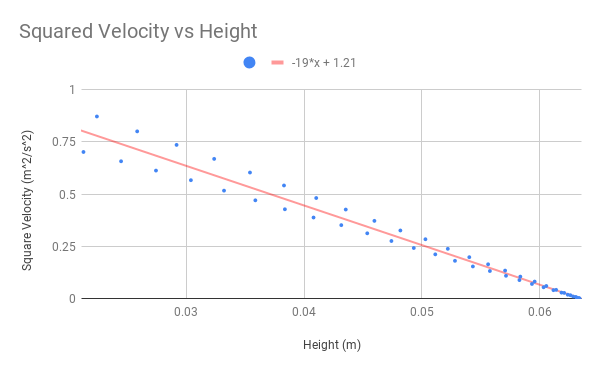
\includegraphics[scale=0.71]{image/07-mechanic/v2-both.png}
    \caption{$v^{2}$ versus $h$ for Run 3: Both upward and downward motion}
    \label{figure:07.v2.3}
\end{figure}
%%%%%%%%%%%%%%%%%%%%%%%%%%%%%%%%%%%%%%%%%%%%%%%%%%%%%%%%%%%%%%%%%%%%%%%%%%%%%%%%
\begin{figure}[ht]
    \centering
    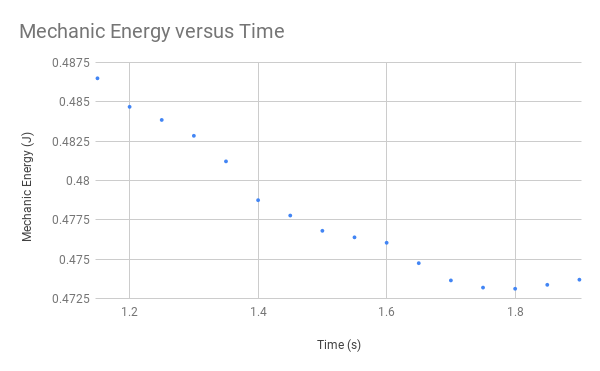
\includegraphics[scale=0.71]{image/07-mechanic/energy-4.png}
    \caption{Mechanic Energy for Run 4: Upward motion only}
    \label{figure.07.run.4.e}
\end{figure}
%%%%%%%%%%%%%%%%%%%%%%%%%%%%%%%%%%%%%%%%%%%%%%%%%%%%%%%%%%%%%%%%%%%%%%%%%%%%%%%%
\begin{figure}[ht]
    \centering
    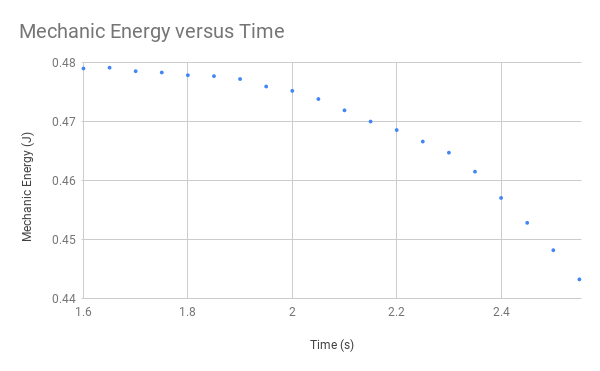
\includegraphics[scale=0.71]{image/07-mechanic/energy-5.png}
    \caption{Mechanic Energy for Run 5: Downward motion only}
    \label{figure.07.run.5.e}
\end{figure}
%%%%%%%%%%%%%%%%%%%%%%%%%%%%%%%%%%%%%%%%%%%%%%%%%%%%%%%%%%%%%%%%%%%%%%%%%%%%%%%%
\begin{figure}[ht]
    \centering
    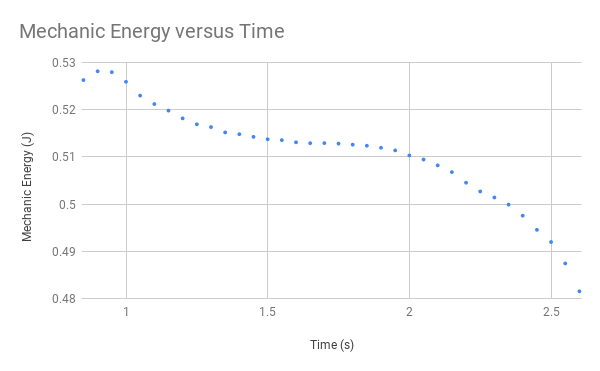
\includegraphics[scale=0.71]{image/07-mechanic/energy-6.png}
    \caption{Mechanic Energy for Run 6: Both upward and downward motion}
    \label{figure.07.run.6.e}
\end{figure}
%%%%%%%%%%%%%%%%%%%%%%%%%%%%%%%%%%%%%%%%%%%%%%%%%%%%%%%%%%%%%%%%%%%%%%%%%%%%%%%%